\documentclass{article}
\usepackage{listings}
\usepackage{graphicx}
\usepackage{graphicx}
\usepackage{subfigure} 
\title{Operational Statistics for SAR Imagery Report}
\author{Huayu Zhang}
\date\today


\begin{document}
	\maketitle
	\section{sample Image} 
	The main purpose of this section is to sample from the original image. The area [1200:1299,3900:3959] in the original image was selected.
	\begin{lstlisting}[frame=tb]
	
	> imagepath <- "../SAR/"
	
	> HH_Complex <- myread.ENVI(paste(imagepath,
	"ESAR97HH.DAT", sep = ""), 
	paste(imagepath, "ESAR97HH.hdr", sep = ""))
	> HH_Intensity <- (Mod(HH_Complex))^2
	> example <- HH_Intensity[1200:1299,3900:3959]
	> vexample <- data.frame(HH=as.vector(example))
	> summary(vexample)
	HH          
	Min.   :    116  
 	1st Qu.: 114391  
 	Median : 296345  
 	Mean   : 473365  
 	3rd Qu.: 618983  
 	Max.   :5365861  
	\end{lstlisting}
	\begin{figure}[htbp]
		\centering
		\subfigure[example.]{
			
\includegraphics[width=5.5cm]{example.png}
			%\caption{fig1}
		}
		\quad
		\subfigure[HistogramExample.]{
			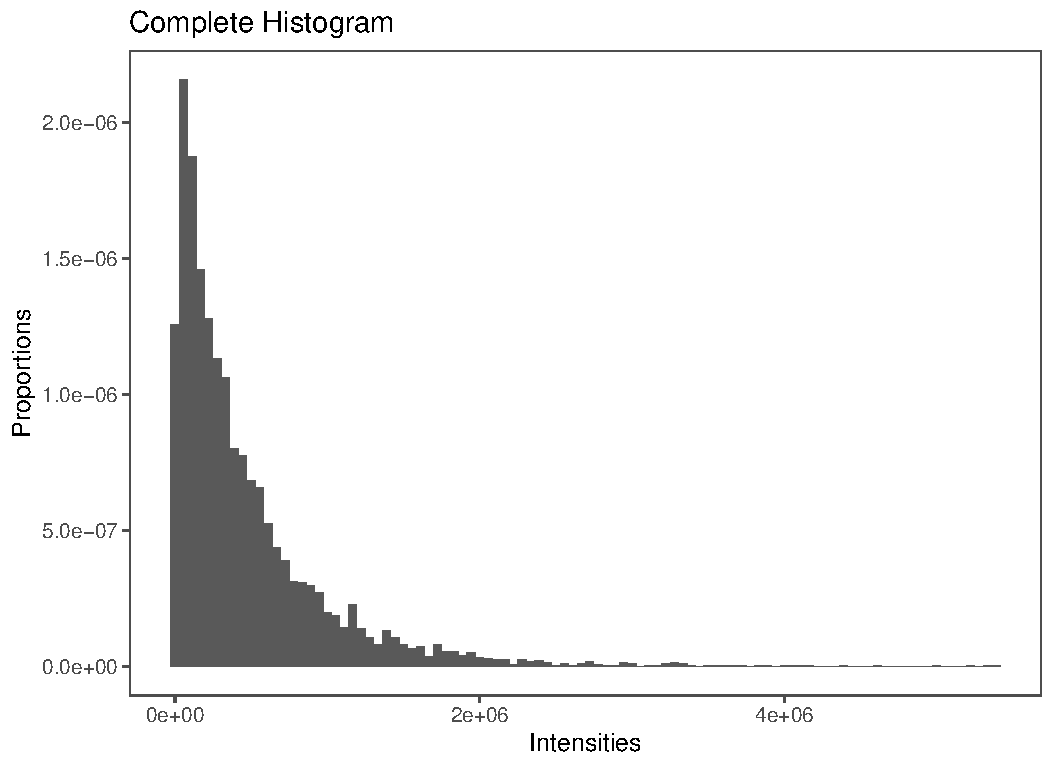
\includegraphics[width=5.5cm]{HistogramExample.pdf}
		}
		\quad
	\end{figure}
	
	\section{Histogram}
	Displaying a histogram of the statistics of the selected area in this section. 
	\begin{lstlisting}[frame=tb]
	> binwidth_complete <- 2*IQR(vexample$HH)*length(vexample$HH)^(-1/3)
	> ggplot(data=vexample, aes(x=HH)) + 
	+   geom_histogram(aes(y=..density..), 
	+                  binwidth = binwidth_complete) + 
	+   xlab("Intensities") +
	+   ylab("Proportions") +
	+   ggtitle("Complete Histogram") +
	+   theme_few()
	> ggsave(filename = "./HistogramExample.pdf")
	\end{lstlisting}
	
	\section{Estimation}
	Analogy estimation and maximum likelihood estimation for selected regions.
	\subsection{analogy}
	\begin{lstlisting}[frame=tb]
	> GI0.Estimator.m1m2 <- function(z, L) {
	+   m1 <- mean(z)
	+   m2 <- mean(z^2)
	+   m212 <- m2/m1^2
	+   
	+   a <- -2 - (L+1) / (L * m212)
	+   g <- m1 * (2 + (L+1) / (L * m212))
	+   
	+   return(list("alpha"=a, "gamma"=g))
	+ }
	\end{lstlisting}
	\begin{lstlisting}[frame=tb]
	> result <- GI0.Estimator.m1m2(example, 1)
	> result
	$alpha
	[1] -2.844684

	$gamma
 	[1] 1346574
	\end{lstlisting}
	\subsection{Likelihood}
	\begin{lstlisting}[frame=tb]
	> LogLikelihoodLknown <- function(params) {
	+   
	+   p_alpha <- -abs(params[1])
	+   p_gamma <- abs(params[2])
	+   p_L <- abs(params[3])
	+   n <- length(vexample$HH)
	+    return(
	+     n*(lgamma(p_L-p_alpha) - p_alpha*log(p_gamma) -
	+        lgamma(-p_alpha)) + (p_alpha-p_L) * 
	+        sum(log(p_gamma + z*p_L)) 
	+   )
	+ }
	\end{lstlisting}
	\begin{lstlisting}[frame=tb]
	> likelihood_result <- maxNR(LogLikelihoodLknown, 
	+                      start=c(result$alpha, result$gamma,1), 
	+                      activePar=c(TRUE,TRUE,FALSE))$estimate[1:2]
	> likelihood_result
	[1] -3.740095e+00  1.346314e+06
	\end{lstlisting}
	
\end{document}
